\documentclass[a4paper]{article}

%% Language and font encodings
\usepackage[english]{babel}
\usepackage[utf8x]{inputenc}
\usepackage[T1]{fontenc}
\usepackage{amsmath}
\usepackage{qtree}
\usepackage{graphicx}

%% Sets page size and margins
\usepackage[a4paper,top=3cm,bottom=2cm,left=3cm,right=3cm,marginparwidth=1.75cm]{geometry}

%% Useful packages
\usepackage{amsmath}
\usepackage{graphicx}
\usepackage[colorinlistoftodos]{todonotes}
\usepackage[colorlinks=true, allcolors=blue]{hyperref}
\title{CS 440 Fall 2018 Homework Assignment 4}
\author{Rafal Stapinski }
\date{November 11 2018}

\begin{document}

\maketitle

\section{}

P(Rain | Clear Forecast) = $\frac{P(Clear Forecast | Rain) P(Rain)}{P(Clear Forecast)}$ \newline
P(Rain | Clear Forecast) = $\frac{.2 * .33}{.33*.2 + .67*.8}$ = 10.96\%

\section{}
The guest should switch. There is a 25\% chance the guest will have chosen a car correctly on the first guess. In that case, switching will result in a 0\% chance of getting the car. However, there is a 50\% the guest picked a goat, and a 25\% chance the guest picked the empty door on the first choice. In both of these conditions, the chance of getting the car if switching is 50\% and the chance of getting the car if staying with the chosen door would be 0\%. This means that staying with the chosen door will only result in a car 25\% of the time, whereas switching would result in a car 37.5\% of the time. 

\section{}
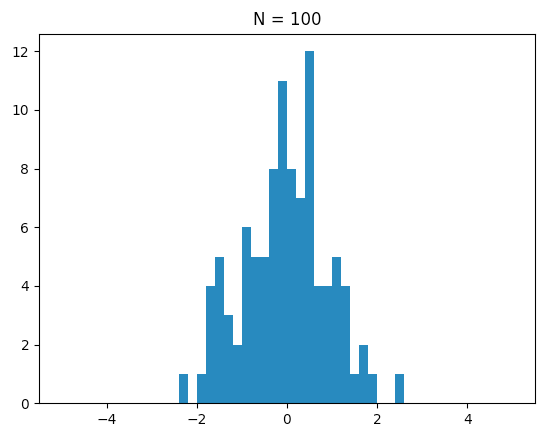
\includegraphics[scale=.4]{100.png}
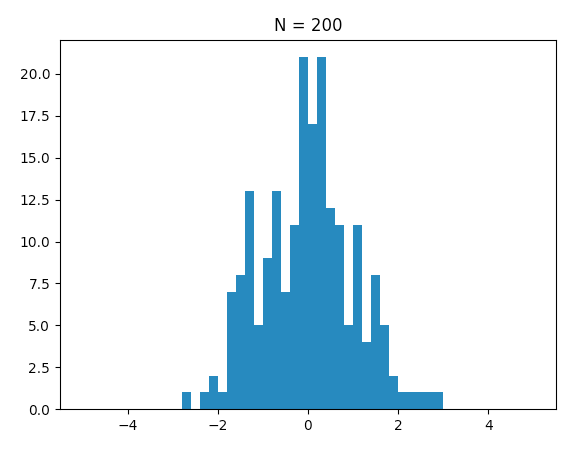
\includegraphics[scale=.4]{200.png}
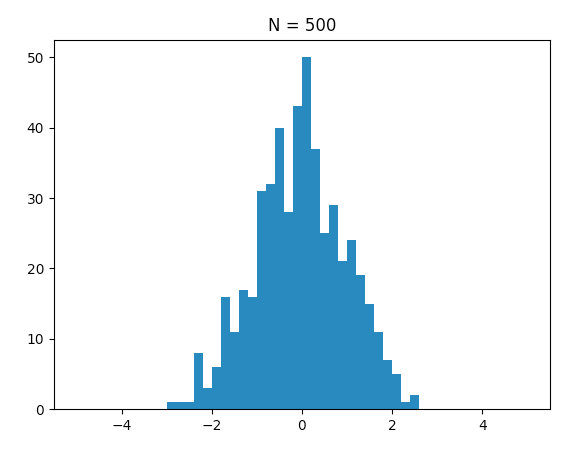
\includegraphics[scale=.4]{500.png}
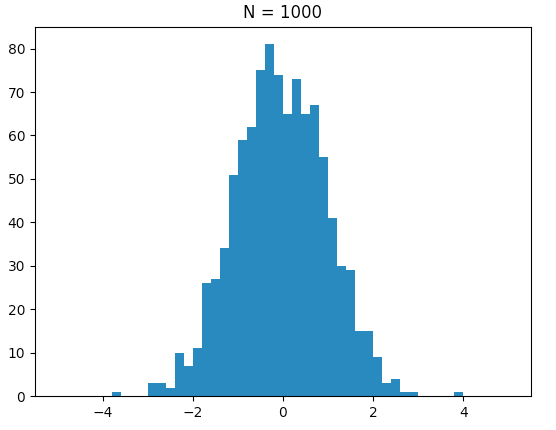
\includegraphics[scale=.4]{1000.png}

\section{}
\subsection{}
P(A,B,C,D,E) = P(A) * P(B) * P(C) * P(D | A,B) * P(E | B,C) =  .2*.5*.8*.1*.3 = 0.0024
\subsection{}
P(A,E | B) = P(A) * [P(C) * P(E | B,C) + P(!C) * P(E | B,!C)] = .2*(.8*.3+.2*.8) = 0.08
\subsection{}
P(A,!B,!C,!D,!E) = P(A) * P(!B) * P(!C) * P(!D | A,!B) * P(!E | !B,!C) = .2*.5*.2*.5*.8 = 0.008
\subsection{}
P(C,!D) | !B) = P(C) * [P(A) * P(!D | A,!B) +  P(!A) * P(!D | !A,!B)] = .8*(.2*.5+.8*.1) = 0.144
\subsection{}
P(B,!C,D | !A) = P(B) * P(!C) * P(D | !A, B) = .5*.2*.6 = 0.06

\section{}
\subsection{}
\subsection{}
\subsection{}
With enumeration: O($n^2$) \newline
With variable elimination: O(n)

\end{document}
